\documentclass[border=14pt]{standalone}
\usepackage{tikz}
\usepackage{lmodern}
\usetikzlibrary{positioning, arrows.meta, fit, backgrounds, calc}

\begin{document}
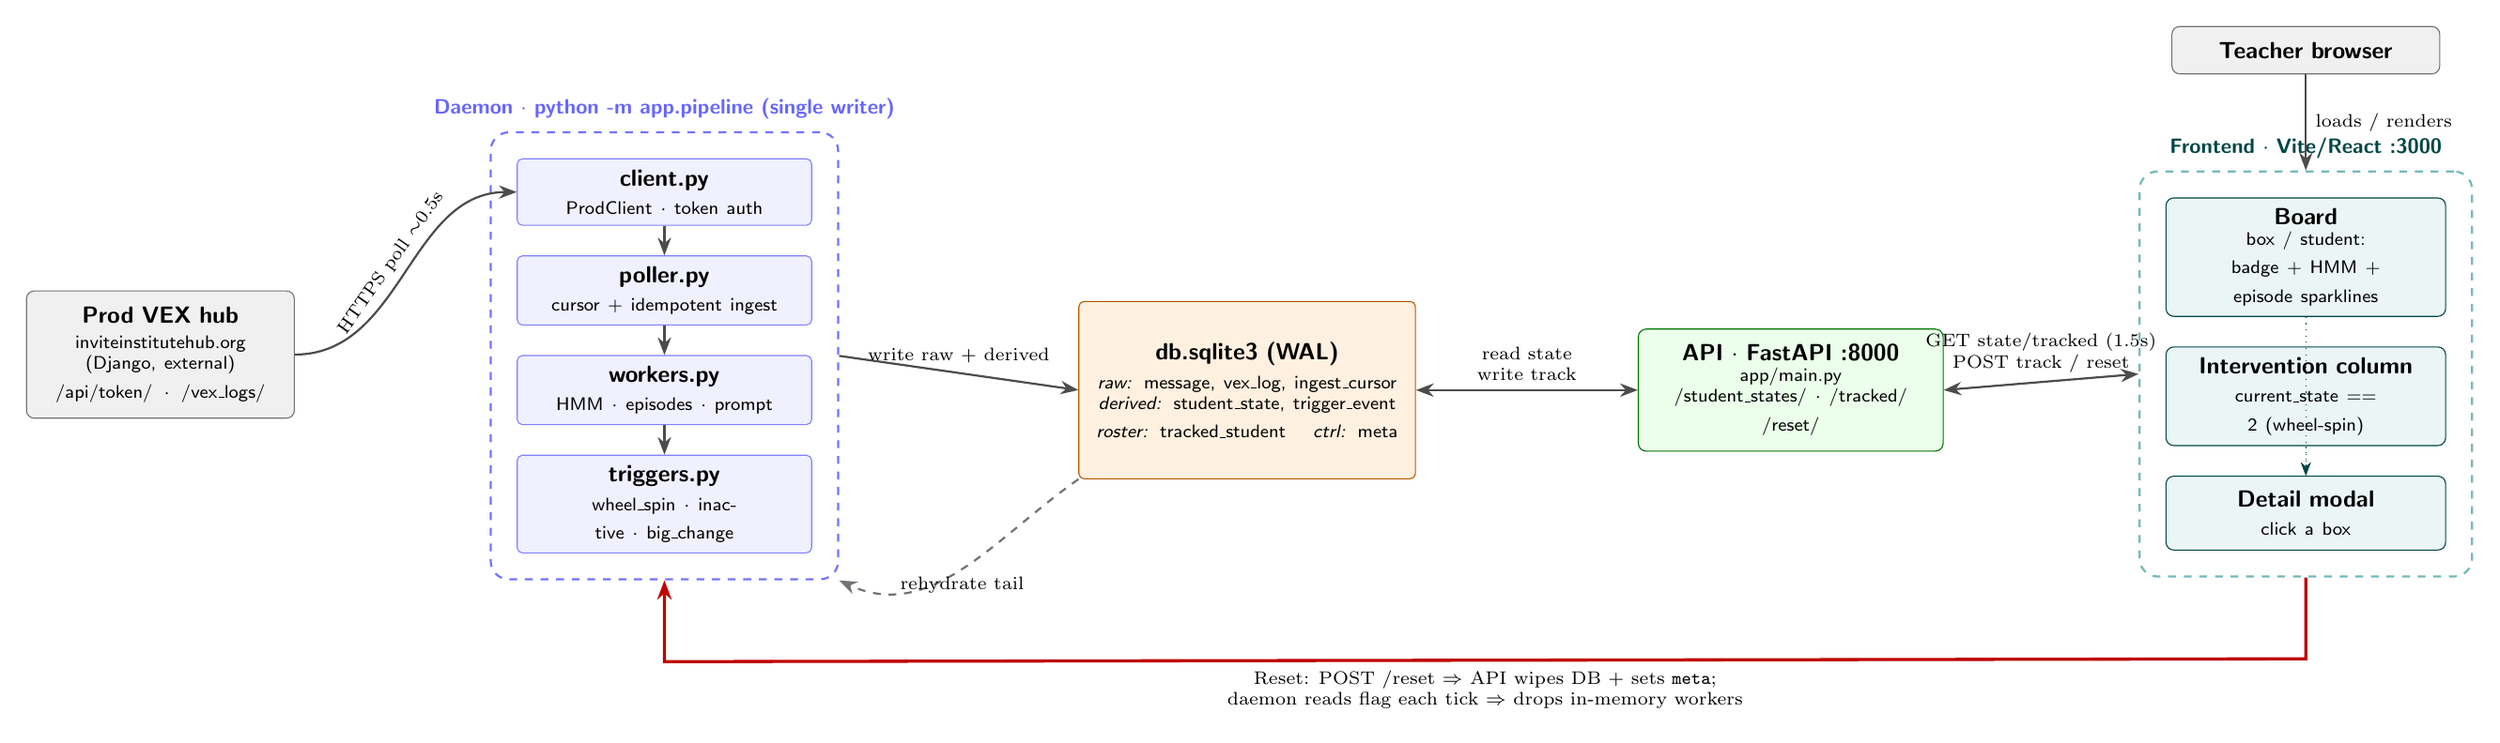
\begin{tikzpicture}[
  font=\sffamily\small, >=Stealth,
  ext/.style  ={rounded corners=3pt, draw=black!55, fill=black!6,  align=center, inner sep=6pt, text width=32mm},
  stage/.style={rounded corners=2pt, draw=blue!50,  fill=blue!6,   align=center, inner sep=4pt, text width=37mm, minimum height=9mm},
  db/.style   ={rounded corners=2pt, draw=orange!70!black, fill=orange!12, align=center, inner sep=5pt, text width=42mm, minimum height=24mm},
  svc/.style  ={rounded corners=3pt, draw=green!45!black, fill=green!8, align=center, inner sep=6pt, text width=37mm, minimum height=14mm},
  pane/.style ={rounded corners=3pt, draw=teal!55!black, fill=teal!8, align=center, inner sep=4pt, text width=35mm, minimum height=10mm},
  grp/.style  ={rounded corners=7pt, draw=#1, thick, dashed, inner sep=10pt},
  flow/.style ={-{Stealth[length=2.4mm]}, thick, draw=black!70},
  bi/.style   ={{Stealth[length=2.4mm]}-{Stealth[length=2.4mm]}, thick, draw=black!70},
  rehy/.style ={-{Stealth[length=2.4mm]}, thick, dashed, draw=black!55},
  reset/.style={-{Stealth[length=2.6mm]}, very thick, draw=red!75!black},
  click/.style={-{Stealth[length=1.8mm]}, dotted, draw=teal!55!black},
]

% ---------- Prod ----------
\node[ext] (prod) {\textbf{Prod VEX hub}\\[2pt]\scriptsize inviteinstitutehub.org\\(Django, external)\\ /api/token/ \,\(\cdot\)\, /vex\_logs/};

% ---------- Daemon (internal stages) ----------
\node[stage, right=30mm of prod, yshift=22mm] (client)   {\textbf{client.py}\\\scriptsize ProdClient \(\cdot\) token auth};
\node[stage, below=4mm of client]             (poller)   {\textbf{poller.py}\\\scriptsize cursor + idempotent ingest};
\node[stage, below=4mm of poller]             (workers)  {\textbf{workers.py}\\\scriptsize HMM \(\cdot\) episodes \(\cdot\) prompt};
\node[stage, below=4mm of workers]            (triggers) {\textbf{triggers.py}\\\scriptsize wheel\_spin \(\cdot\) inactive \(\cdot\) big\_change};
\draw[flow] (client)--(poller); \draw[flow] (poller)--(workers); \draw[flow] (workers)--(triggers);
\begin{scope}[on background layer]
  \node[grp=blue!55, fit=(client)(poller)(workers)(triggers)] (daemon) {};
\end{scope}
\node[blue!60, font=\sffamily\footnotesize\bfseries, above=1pt of daemon] {Daemon \(\cdot\) python -m app.pipeline (single writer)};

% ---------- DB ----------
\node[db, right=36mm of workers] (db) {\textbf{db.sqlite3 (WAL)}\\[3pt]\scriptsize
  \emph{raw:} message, vex\_log, ingest\_cursor\\
  \emph{derived:} student\_state, trigger\_event\\
  \emph{roster:} tracked\_student \quad \emph{ctrl:} meta};

% ---------- API ----------
\node[svc, right=30mm of db] (api) {\textbf{API \(\cdot\) FastAPI :8000}\\\scriptsize app/main.py\\ /student\_states/ \(\cdot\) /tracked/\\ /reset/};

% ---------- Frontend (panes) ----------
\node[pane, right=30mm of api, yshift=18mm] (board) {\textbf{Board}\\\scriptsize box / student:\\ badge + HMM + episode sparklines};
\node[pane, below=4mm of board]             (col)   {\textbf{Intervention column}\\\scriptsize current\_state == 2 (wheel-spin)};
\node[pane, below=4mm of col]               (modal) {\textbf{Detail modal}\\\scriptsize click a box};
\draw[click] (board) -- (modal); \draw[click] (col) -- (modal);
\begin{scope}[on background layer]
  \node[grp=teal!55, fit=(board)(col)(modal)] (fe) {};
\end{scope}
\node[teal!55!black, font=\sffamily\footnotesize\bfseries, above=1pt of fe] {Frontend \(\cdot\) Vite/React :3000};

% ---------- Browser ----------
\node[ext, above=13mm of fe] (browser) {\textbf{Teacher browser}};

% ---------- flows ----------
\draw[flow] (prod.east) to[out=0,in=180] node[above, font=\scriptsize, sloped]{HTTPS poll \(\sim\)0.5s} (client.west);
\draw[flow] (daemon.east) -- node[above, font=\scriptsize]{write raw + derived} (db.west);
\draw[rehy] (db.south west) to[out=215,in=-25] node[below, font=\scriptsize]{rehydrate tail} (daemon.south east);
\draw[bi]   (db.east) -- node[above, font=\scriptsize, align=center]{read state\\ write track} (api.west);
\draw[bi]   (api.east) -- node[above, font=\scriptsize, align=center]{GET state/tracked (1.5s)\\ POST track / reset} (fe.west);
\draw[flow] (browser.south) -- node[right, font=\scriptsize]{loads / renders} (fe.north);

% ---------- reset signal (red, shallow orthogonal channel under the spine) ----------
\draw[reset] (fe.south) -- ($(fe.south)+(0,-11mm)$)
  -- node[below, font=\scriptsize, align=center]
       {Reset: POST /reset \(\Rightarrow\) API wipes DB + sets \texttt{meta};\\
        daemon reads flag each tick \(\Rightarrow\) drops in-memory workers}
     ($(daemon.south)+(0,-11mm)$)
  -- (daemon.south);

\end{tikzpicture}
\end{document}
